\subsection{Android Testapplikation Bildschirme und Activities \label{anhang:test_app_screens}}
\begin{figure}[htb]
	\centering
	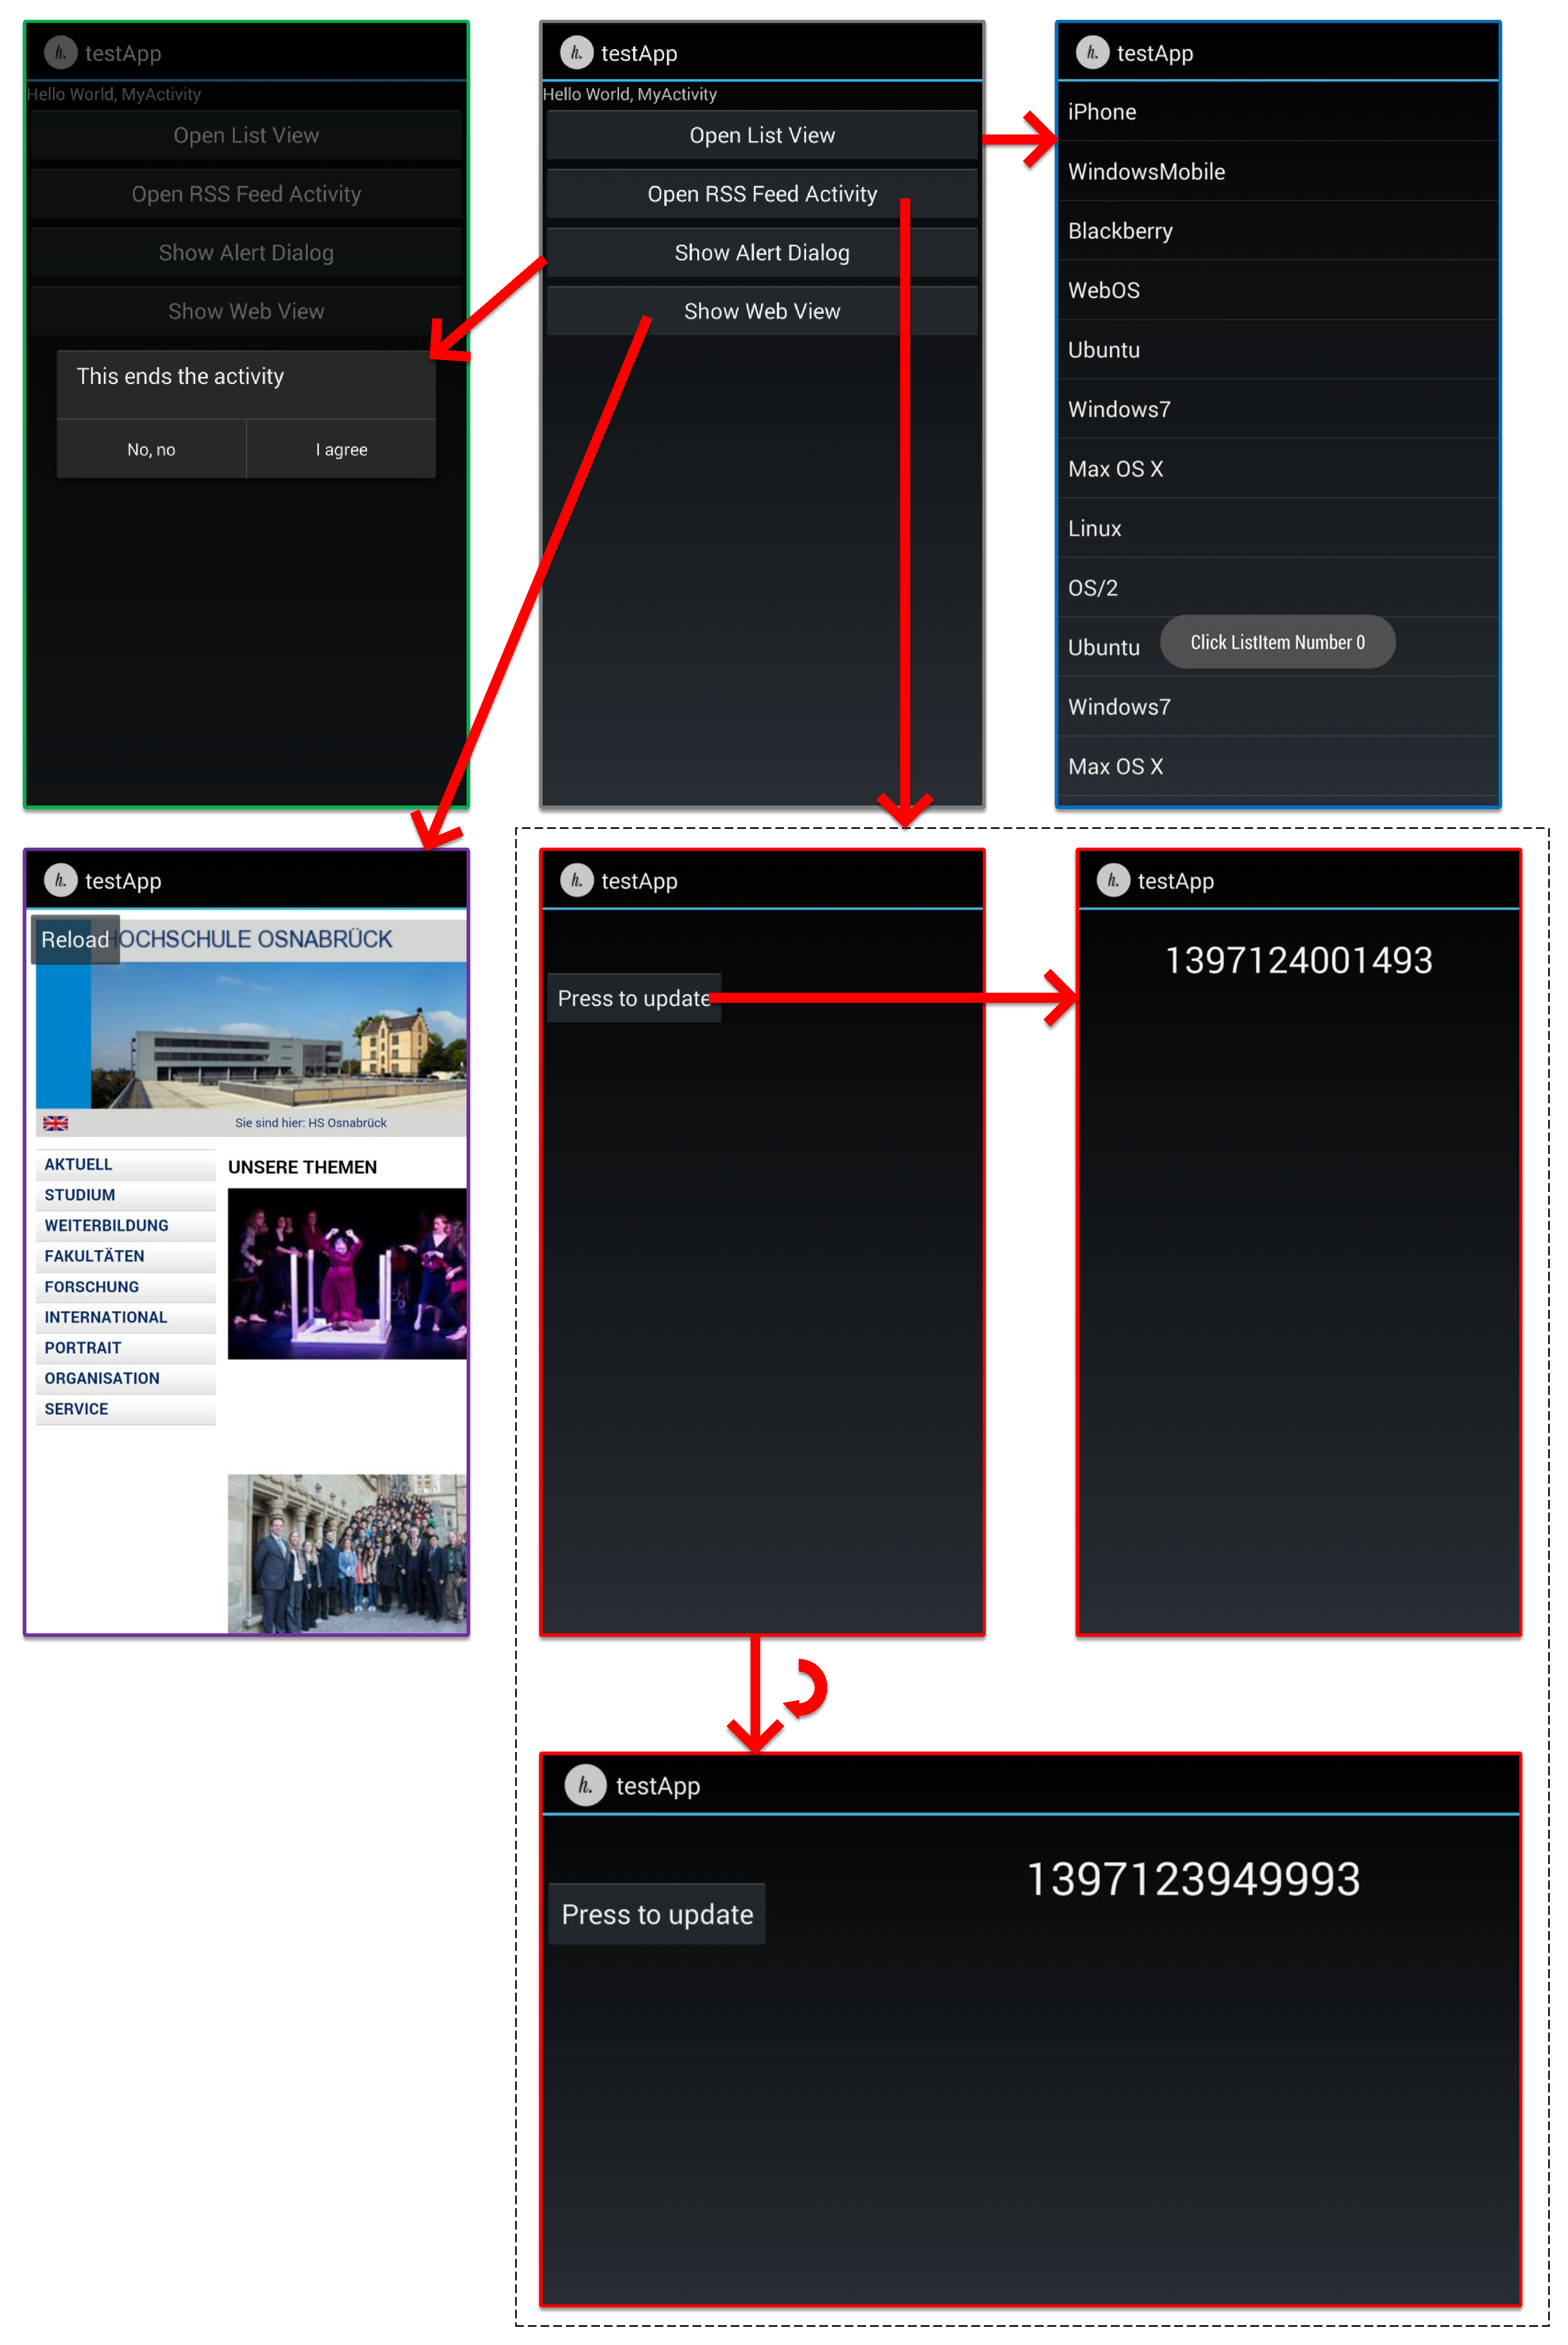
\includegraphics[width=0.7\linewidth]{img/client_test_app_screens}
	\caption{Bildschirme der Testapplikation mit farblich markierten Activities. \label{fig:client_test_app_screens}}
\end{figure}

\newpage

\subsection{ER-Diagramm Datenbank\label{apdx:db}}

\begin{figure}[h!]
	\centering
	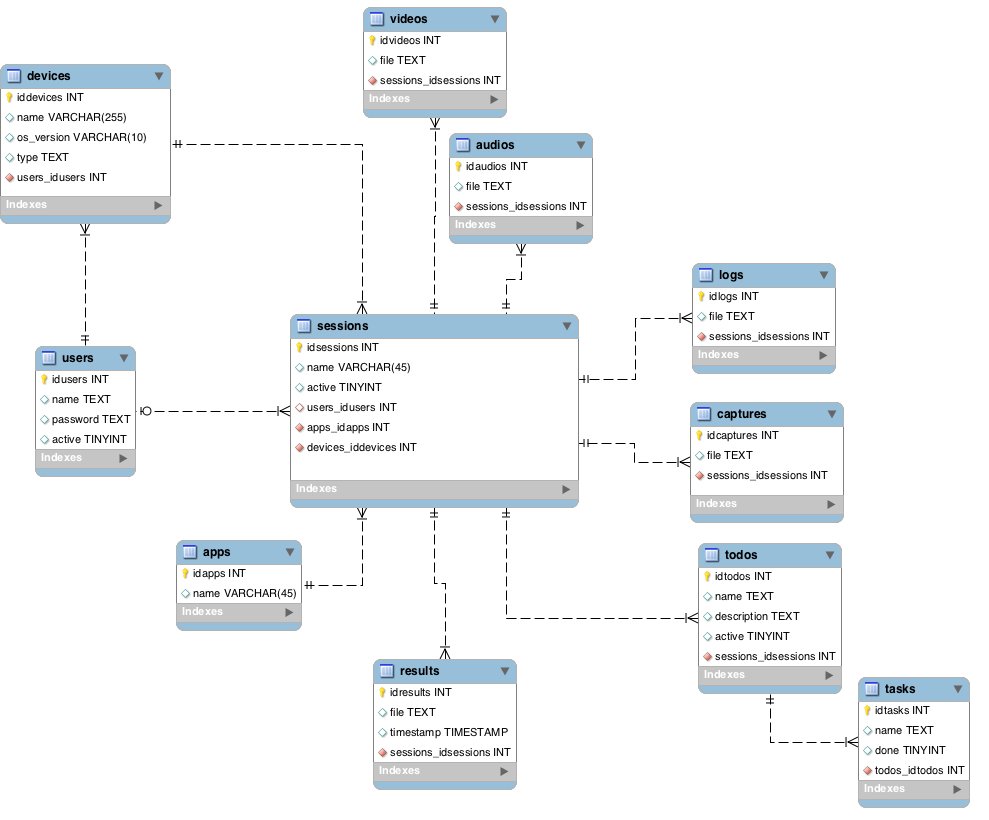
\includegraphics[width=\linewidth,keepaspectratio]{img/db_model.png}
	\caption{Datenbank Modell}
	\label{figure-db-model}
\end{figure}
\newpage

\subsection{Screenshots des webbasierten Verwaltungswerkzeugs}
\label{anhang:screens-webtool}

\begin{figure}[h!]
	\centering
		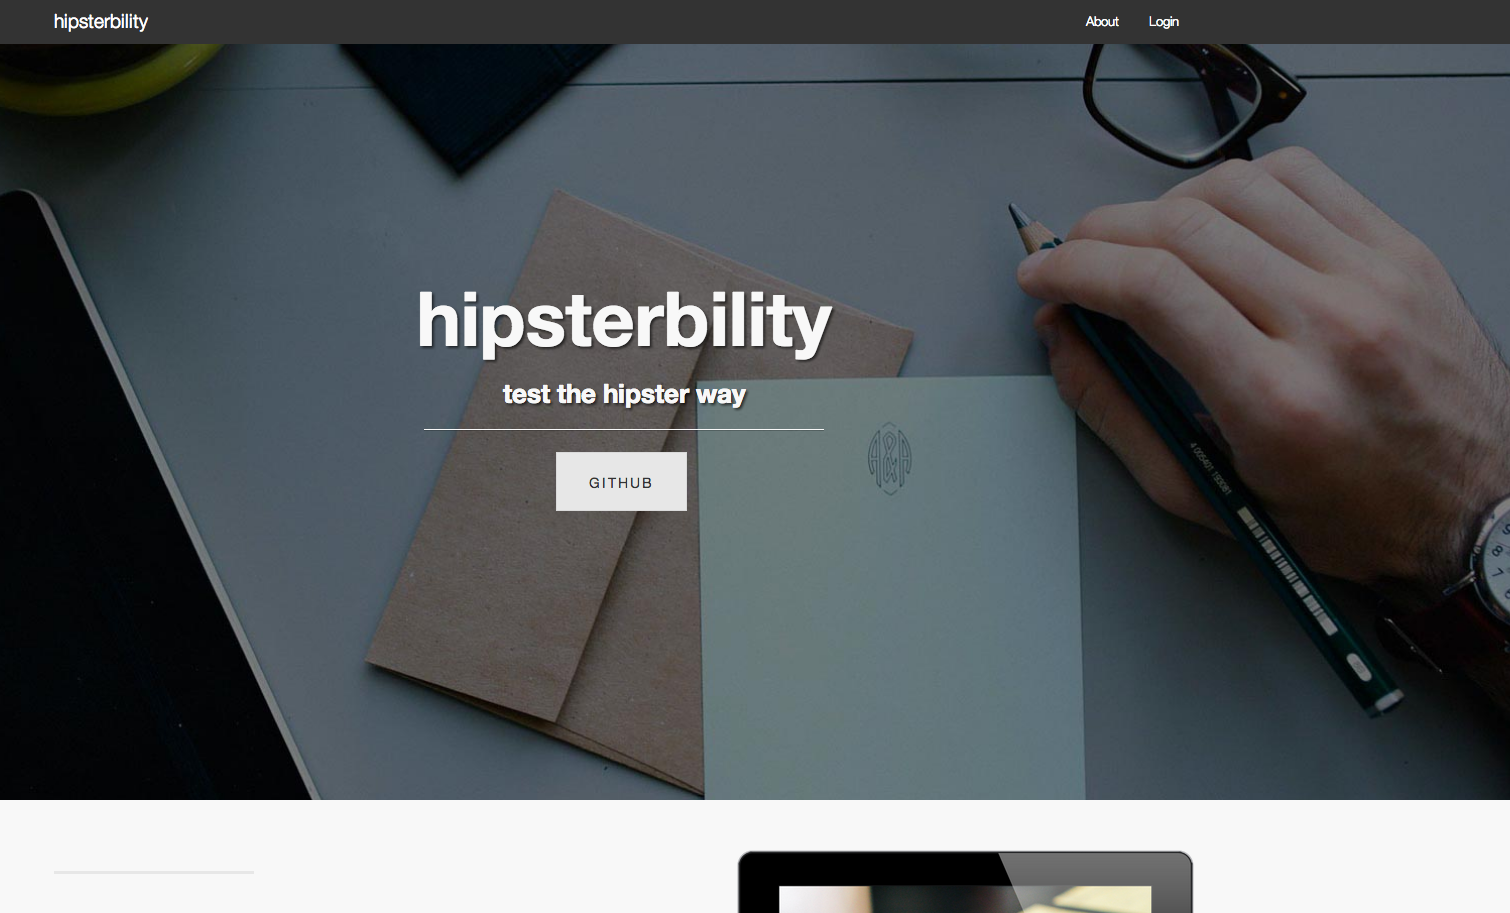
\includegraphics[width=\linewidth,keepaspectratio]{img/index-page.png}
	\caption{Index-Seite der Anwendung}
	\label{fig: index-page}
\end{figure}

\begin{figure}[h!]
	\centering
		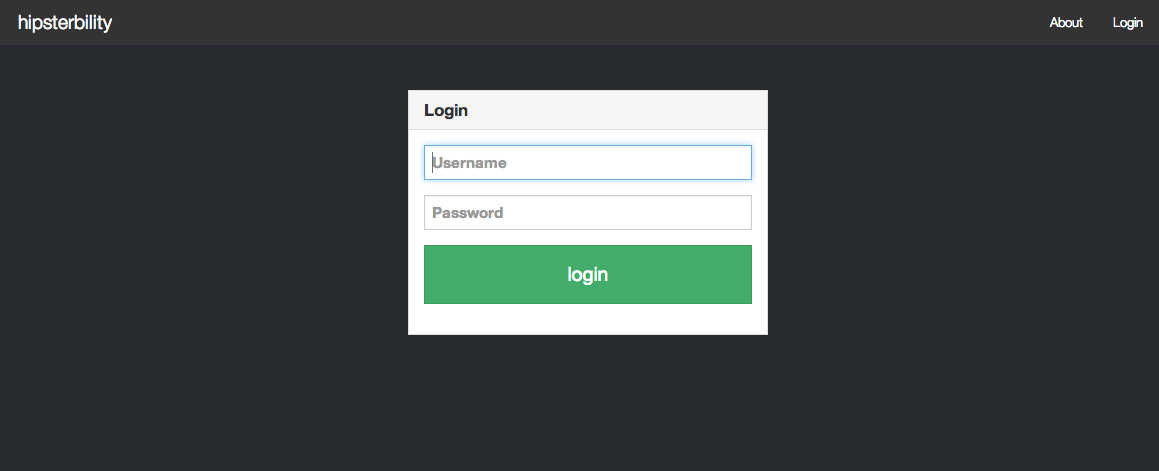
\includegraphics[width=\linewidth,keepaspectratio]{img/login-page.png}
	\caption{Login-Seite der Anwendung}
	\label{fig: login-page}
\end{figure}
\newpage
\begin{figure}[h!]
	\centering
		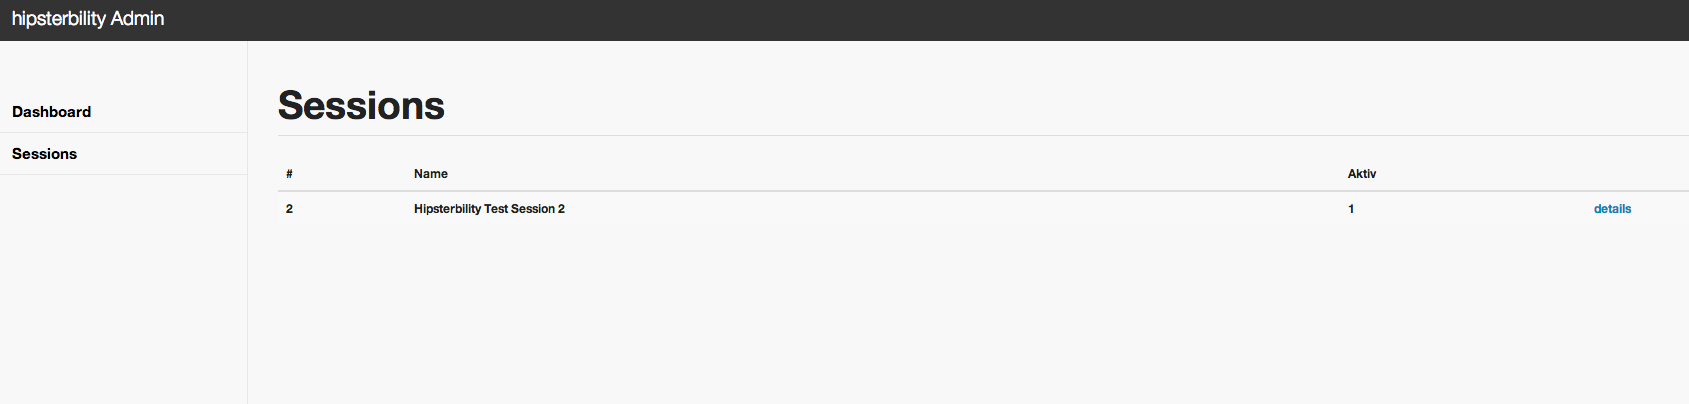
\includegraphics[width=\linewidth,keepaspectratio]{img/sessions-page.png}
	\caption{Listenansicht für Testsessions}
	\label{fig: sessions-page}
\end{figure}

\begin{figure}[h!]
	\centering
		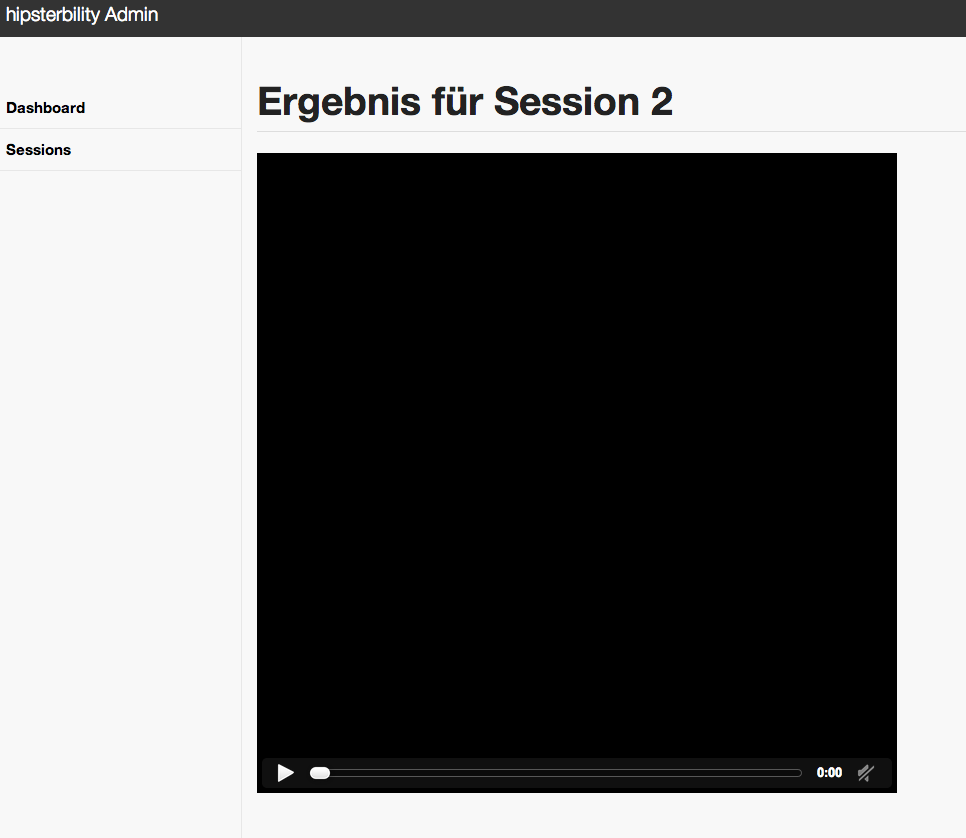
\includegraphics[width=\linewidth,keepaspectratio]{img/session-result-page.png}
	\caption{Web-Ansicht der Ergebnisse}
	\label{fig: session-result-page}
\end{figure}
\newpage
\begin{figure}[h!]
	\centering
		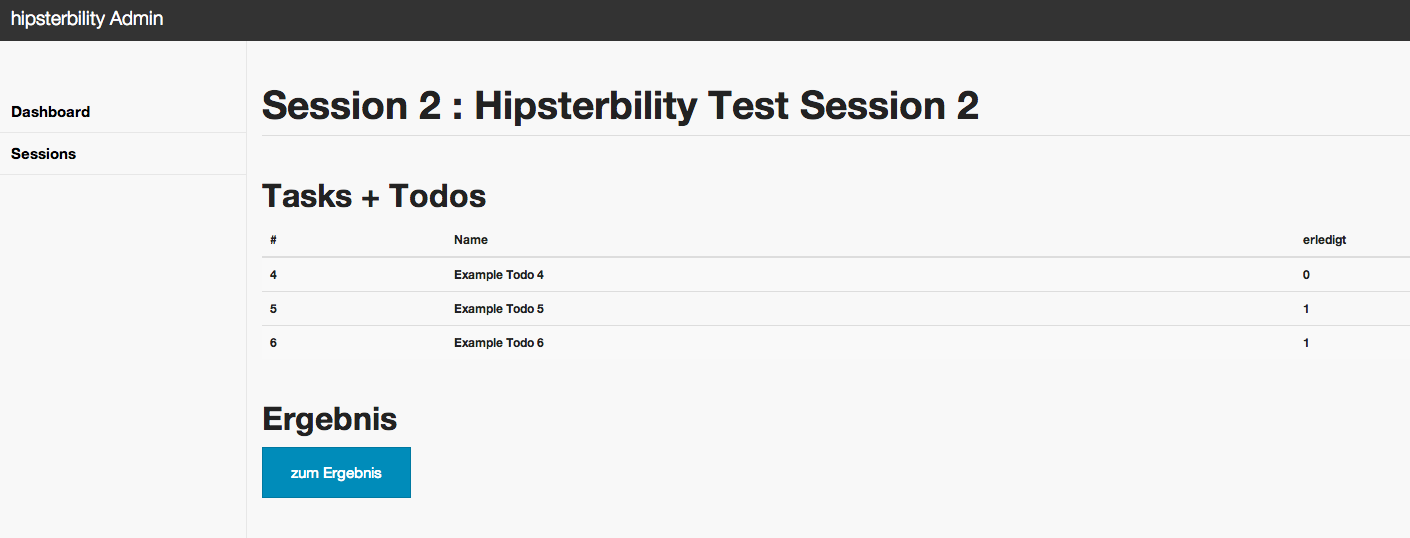
\includegraphics[width=\linewidth,keepaspectratio]{img/session-detail-page.png}
	\caption{Detailansicht einer Testsession}
	\label{fig: session-detail-page}
\end{figure}

\begin{figure}[h!]
	\centering
		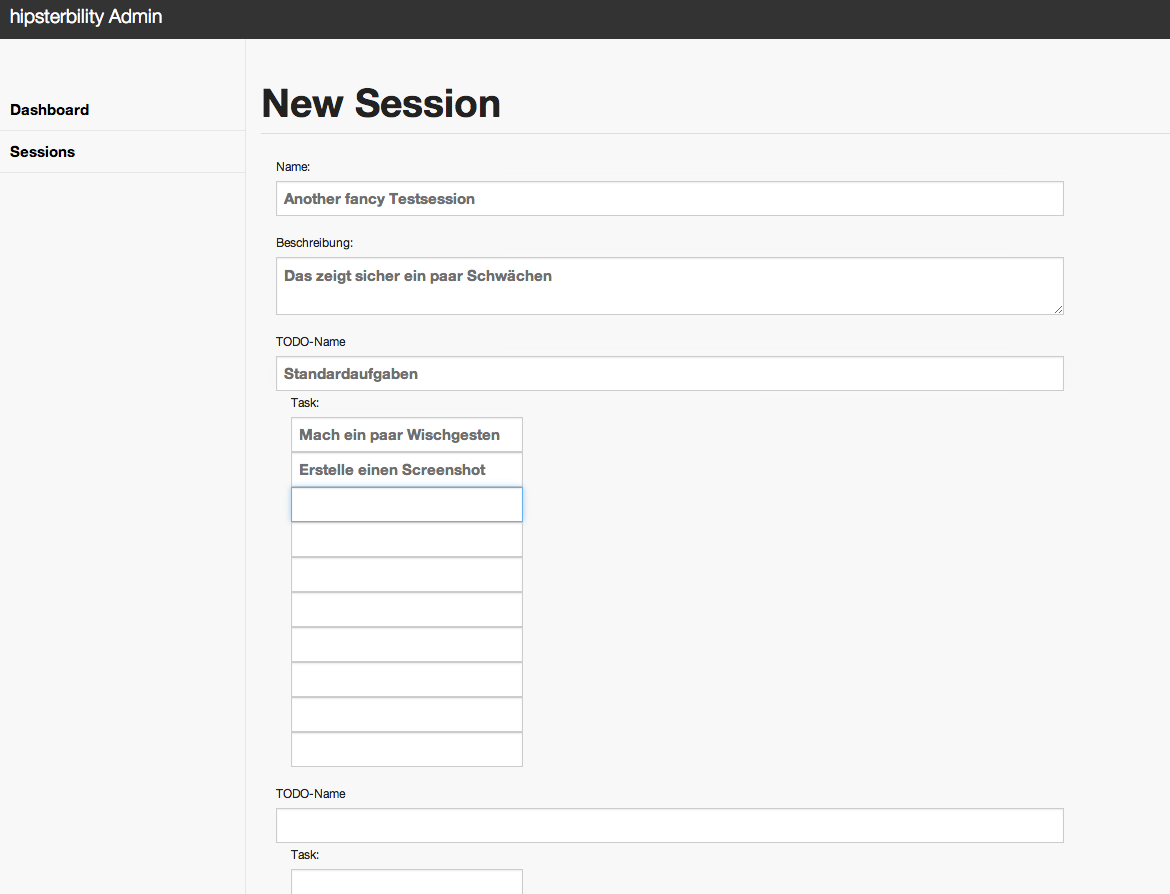
\includegraphics[width=\linewidth,keepaspectratio]{img/session-create-page.png}
	\caption{Neue Session anlegen}
	\label{fig: session-create-page}
\end{figure}

\newpage

\subsection{IntelliJ Idea\label{apdx:intellij}}
\begin{figure}[h!]
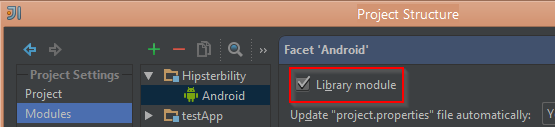
\includegraphics[width=\linewidth]{img/screen_intellij_library_module}
\caption{Library module in IntelliJ IDEA aktivieren (Screenshot)}
\label{fig:screen_intellij_library_module}
\end{figure}

\begin{figure}[h!]
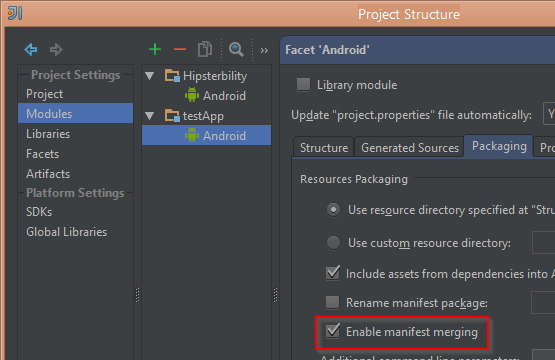
\includegraphics[width=\linewidth]{img/screen_intellij_manifest_merging}
\caption{Manifest merging in IntelliJ IDEA aktivieren (Screenshot)}
\label{fig:screen_intellij_maifest_merging}
\end{figure}